\documentclass[11pt,a4paper]{article}

% Pacotes essenciais
\usepackage[utf8]{inputenc}
\usepackage[T1]{fontenc}
\usepackage{lmodern}
\usepackage[portuguese]{babel}
\usepackage{graphicx}
\usepackage{amsmath}
\usepackage{amsfonts}
\usepackage{amssymb}
\usepackage{float}
\usepackage{caption}
\usepackage{subcaption}
\usepackage{xcolor}
\usepackage{colortbl}
\usepackage{fancyhdr}
\usepackage{geometry}
\usepackage{titlesec}
\usepackage{lipsum}
\usepackage[alf]{abntex2cite}
\usepackage{booktabs}
\usepackage{array}
\usepackage{enumitem}
\usepackage{tikz}
\usetikzlibrary{shapes.geometric}
\usepackage[hidelinks]{hyperref}
\usetikzlibrary{positioning}

% Definição das cores
\definecolor{headercolor}{HTML}{b11116}
\definecolor{secondarycolor}{HTML}{3a5461}

% Configuração da página
\geometry{
    a4paper,
    top=2.8cm,
    bottom=2.5cm,
    left=2.5cm,
    right=2.5cm,
    headheight=1.2cm,
    headsep=0.5cm
}

% Configuração do cabeçalho
\pagestyle{fancy}
\fancyhf{}
\renewcommand{\headrulewidth}{0pt}
\renewcommand{\footrulewidth}{0.5pt}

\fancyhead[L]{%
    \begin{tikzpicture}[remember picture, overlay]
        \fill[headercolor] (current page.north west) rectangle ([yshift=-1.2cm]current page.north east);
        \node[anchor=west, inner sep=0pt] at ([xshift=1cm, yshift=-0.6cm]current page.north west) 
            {
\includegraphics[height=0.8cm]{imgs/base/fatec-rgt.png}};
        \node[anchor=east, inner sep=0pt] at ([xshift=-1cm, yshift=-0.6cm]current page.north east) 
            {
\includegraphics[height=0.9cm]{imgs/base/cps-logo.png}};
        \node[anchor=east, inner sep=0pt] at ([xshift=-2.8cm, yshift=-0.6cm]current page.north east) 
            {
\includegraphics[height=1.05cm]{imgs/base/governo-sp-secretaria-logo.png}};
    \end{tikzpicture}
}

\fancyfoot[L]{\footnotesize\textcolor{secondarycolor}{Faculdade de Tecnologia do Estado de São Paulo\\ fatecregistro.cps.sp.gov.br}}
\fancyfoot[R]{\thepage}

% Configuração dos títulos das seções
\titleformat{\section}
    {\normalfont\large\bfseries\color{secondarycolor}}
    {\thesection}{1em}{}

\titleformat{\subsection}
    {\normalfont\normalsize\bfseries\color{secondarycolor}}
    {\thesubsection}{1em}{}

\begin{document}

% ===== CAPA =====
\begin{titlepage}
    \centering
    
    % Logos no topo
    \begin{tikzpicture}[remember picture, overlay]
        \fill[headercolor] (current page.north west) rectangle ([yshift=-1.2cm]current page.north east);
        \node[anchor=west, inner sep=0pt] at ([xshift=1cm, yshift=-0.6cm]current page.north west) 
            {
\includegraphics[height=0.8cm]{imgs/base/fatec-rgt.png}};
        \node[anchor=east, inner sep=0pt] at ([xshift=-1cm, yshift=-0.6cm]current page.north east) 
            {
\includegraphics[height=0.9cm]{imgs/base/cps-logo.png}};
        \node[anchor=east, inner sep=0pt] at ([xshift=-2.8cm, yshift=-0.6cm]current page.north east) 
            {
\includegraphics[height=1.05cm]{imgs/base/governo-sp-secretaria-logo.png}};
    \end{tikzpicture}
    
    \vspace*{3.5cm}
    
    % Nome da faculdade
    {\normalsize FACULDADE DE TECNOLOGIA DO ESTADO DE SÃO PAULO\par}
    \vspace{0.5cm}
    
    % Curso
    {\normalsize DESENVOLVIMENTO DE SOFTWARE MULTIPLATAFORMA\par}
    
    \vspace{4cm}
    
    % Artefatos do Projeto de Software
    {\normalsize ARTEFATOS DO PROJETO DE SOFTWARE\par}
    
    \vspace{0.3cm}
    
    % Nome do projeto
    {\normalsize Plataforma IoT de Monitoramento para Criação de Bubalinos\par}
    
    \vspace{3cm}
    
    % Autores
    {\normalsize
    Arthur Fukunaga\\
    Leo De Lima\\
    Matheus Ferrari\\
    Vinícius Souza\\
    }
    
    \vfill
    
    % Rodapé
    {\small Registro -- SP\\
    2026}
    
\end{titlepage}

% Força o cabeçalho em todas as páginas
\pagestyle{fancy}

% ===== SUMÁRIO =====
\tableofcontents
\newpage

\subsection*{Lista de Artefatos e suas Finalidades}

\begin{itemize}
    \item \textbf{CANVAS:} Modelo de negócio e estratégia
    \item \textbf{SWOT:} Análise estratégica de forças, fraquezas, oportunidades e ameaças
    \item \textbf{UX/UI:} Design de interface e experiência do usuário
    \item \textbf{Website:} Estrutura e especificações técnicas web
     \item \textbf{Aplicação:} Funcionalidades, arquitetura e tecnologias utilizadas no sistema
    \item \textbf{Diagramas UML:} Modelagem visual do sistema
    \item \textbf{Diagramas de Banco de Dados:} Modelagem visual do sistema
    \item \textbf{DevOps:} Infraestrutura, automação e práticas de entrega contínua
\end{itemize}

\vspace{0.5cm}
\noindent\rule{\textwidth}{0.5pt}

\newpage

% ===== CANVAS =====
\section{CANVAS: Modelo de Negócio e Estratégia}

O Business Model Canvas \cite{santos2024} é uma ferramenta visual estratégica\footnote{O Canvas foi desenvolvido por Alexander Osterwalder e é amplamente utilizado em startups e empresas estabelecidas para modelagem de negócios.} que permite descrever, analisar e projetar modelos de negócio de forma clara e objetiva. O canvas é dividido em nove blocos fundamentais que cobrem as principais áreas de um negócio.

\begin{table}[H]
\centering
\caption{Business Model Canvas -- Visão Geral}
\label{tab:canvas}
\small
\begin{tabular}{|p{2.5cm}|p{2.5cm}|p{2.8cm}|p{2.5cm}|p{2.8cm}|}
\end{tabular}
\end{table}

\begin{figure}[H]
\centering
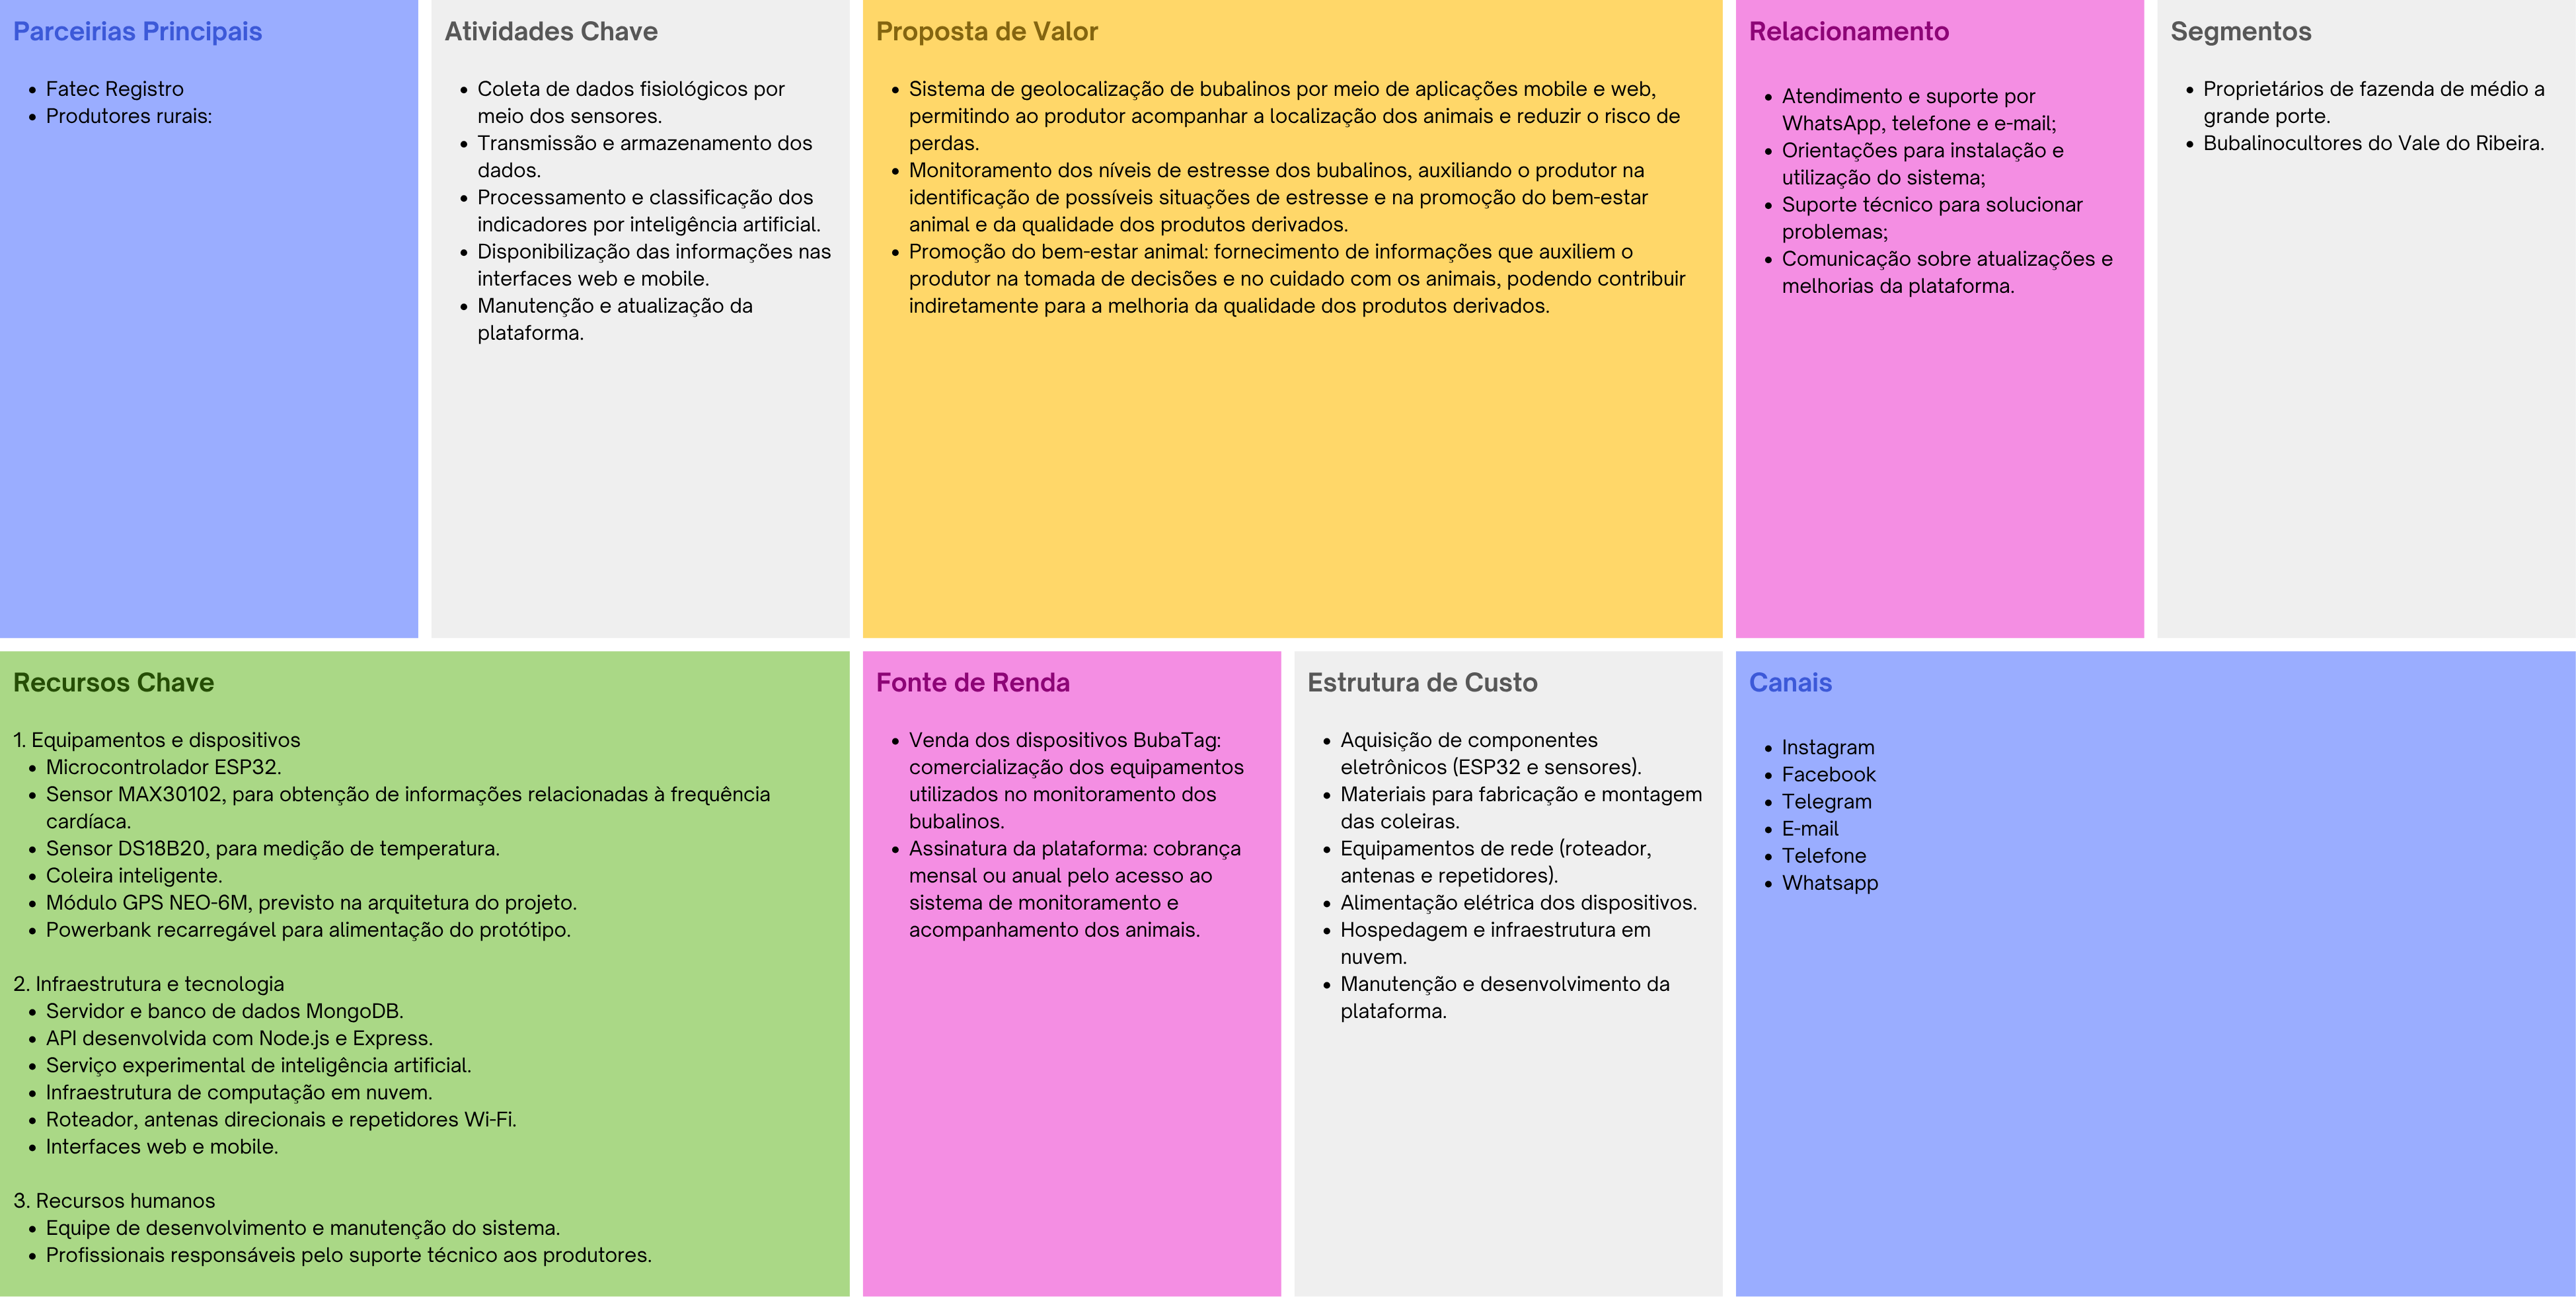
\includegraphics[width=\textwidth]{imgs/bubatag/Canva.png}
\caption{Business Model Canvas do Projeto}
\label{fig:canvas}
\end{figure}


% ===== SWOT =====
\section{SWOT: Análise Estratégica}

A Análise SWOT (Strengths, Weaknesses, Opportunities, Threats) ou FOFA (Forças, Oportunidades, Fraquezas e Ameaças) \cite{oliveira2023} é uma ferramenta fundamental para planejamento estratégico\footnote{A análise SWOT foi criada na década de 1960 por Albert Humphrey no Stanford Research Institute.} que permite identificar fatores internos e externos que impactam o projeto. Analisa forças, fraquezas, oportunidades e ameaças do projeto.



A matriz SWOT pode ser apresentada em formato de tabela conforme o exemplo abaixo:

\begin{table}[H]
\centering
\caption{Análise SWOT do Projeto}
\label{tab:swot}
\begin{tabular}{|p{7.2cm}|p{7.2cm}|}

\begin{figure}[H]
\centering
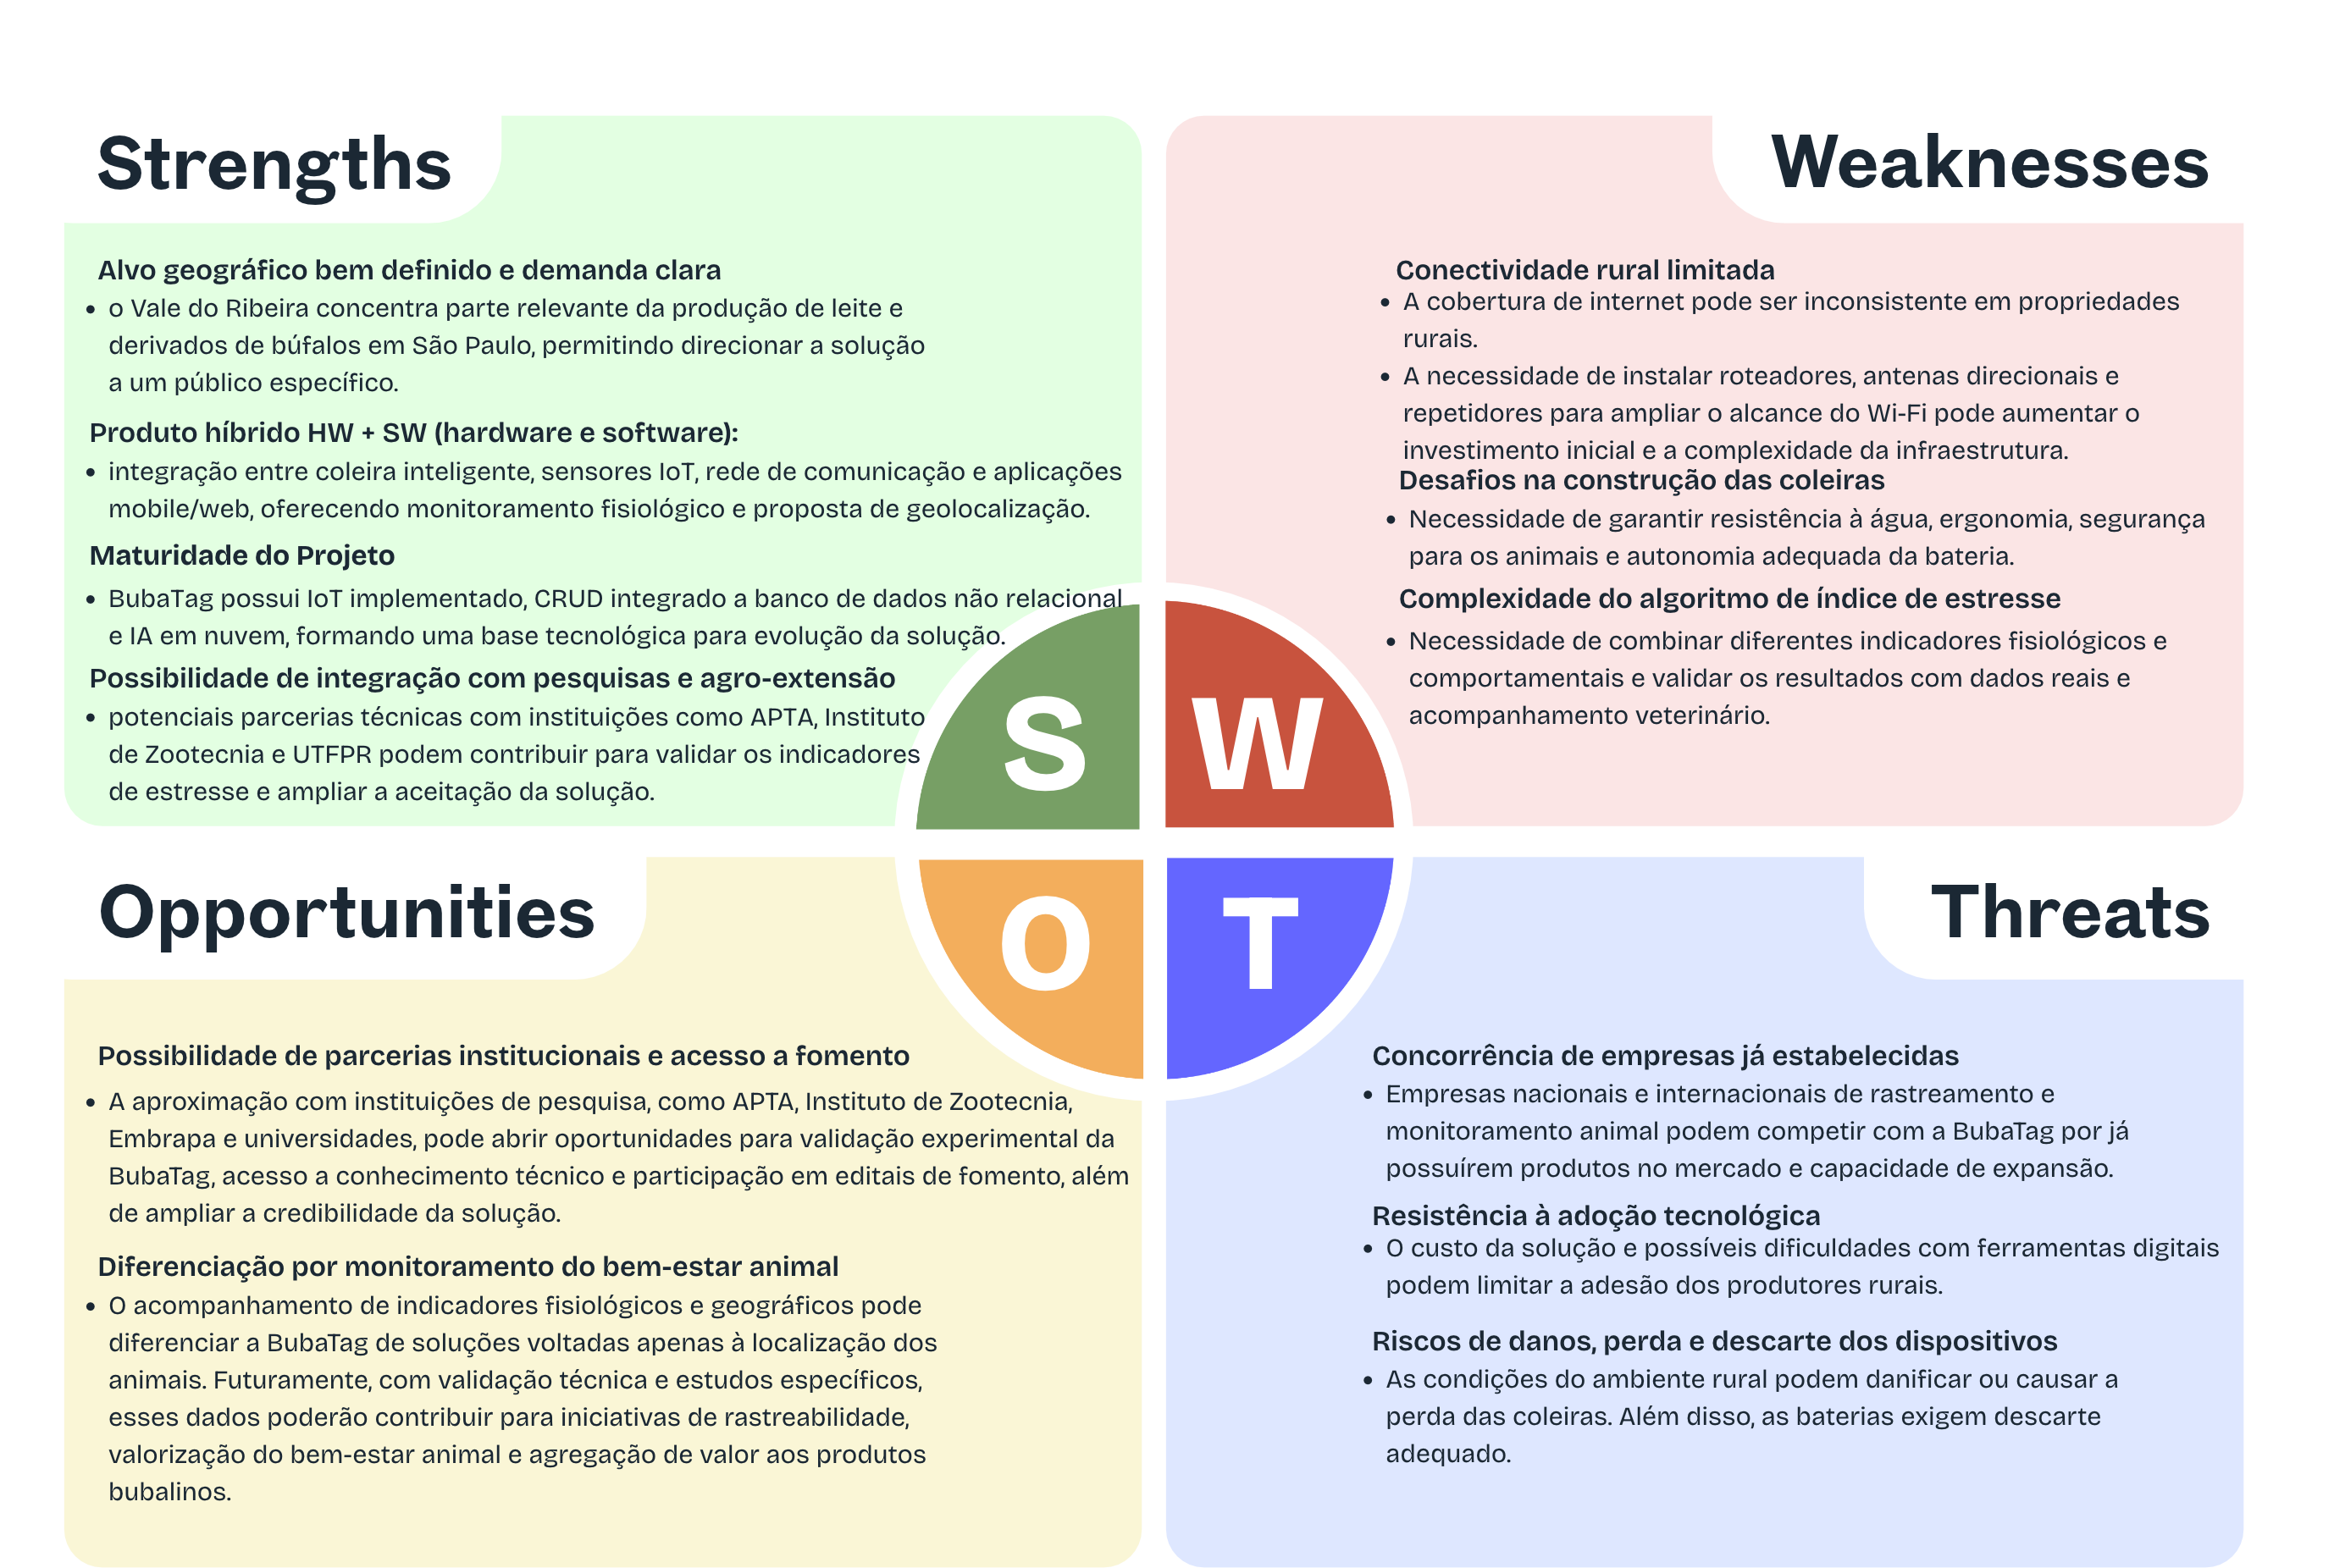
\includegraphics[width=\textwidth]{imgs/bubatag/SWOT.png}
\caption{Análise SWOT do Projeto}
\label{fig:canvas}
\end{figure}

\end{tabular}
\end{table}

\subsection{Recomendações Estratégicas}

Com base na análise SWOT, as principais estratégias devem focar em:
\begin{itemize}
    \item \textbf{Forças + Oportunidades:} Investir no marketing digital para aproveitar o crescimento do mercado
    \item \textbf{Forças + Ameaças:} Reforçar a segurança para se diferenciar da concorrência
    \item \textbf{Fraquezas + Oportunidades:} Buscar parcerias para ampliar a presença no mercado
    \item \textbf{Fraquezas + Ameaças:} Criar planos de contingência e melhorar a documentação
\end{itemize}

% ===== UX/UI =====
\section{UX/UI: Design de Interface e Experiência do Usuário}

UX (User Experience) e UI (User Interface) \cite{silva2025} são disciplinas complementares focadas em criar produtos digitais que sejam funcionais, acessíveis e agradáveis de usar.\footnote{Ferramentas populares para design UX/UI incluem Figma, Adobe XD, Sketch e InVision.} O UX concentra-se na experiência geral do usuário, enquanto o UI cuida dos elementos visuais e interativos.


\subsection{Guia de Estilos}

É importante documentar o design system utilizado:

\begin{table}[H]
\centering
\caption{Paleta de Cores do Site da Equipe}
\label{tab:cores-equipe}

\begin{tabular}{|l|c|l|p{4cm}|}
\hline
\textbf{Elemento} & \textbf{Cor} & \textbf{Código HEX} & \textbf{Uso} \\
\hline

Primária & \colorbox[HTML]{E38B18}{\phantom{AAA}} & \#E38B18 & Destaques e títulos \\

Secundária & \colorbox[HTML]{12C400}{\phantom{AAA}} & \#12C400 & Botões e ações \\

Fundo Principal & \colorbox[HTML]{ECECEC}{\phantom{AAA}} & \#ECECEC & Fundo das páginas \\

Fundo Secundário & \colorbox[HTML]{3F3F3F}{\phantom{AAA}} & \#3F3F3F & Navbar e cards \\

Texto Principal & \colorbox[HTML]{111111}{\color{white}\phantom{AAA}} & \#111111 & Textos principais \\

Texto Secundário & \colorbox[HTML]{FFFFFF}{\color{black}\phantom{AAA}} & \#FFFFFF & Textos em destaque \\

Sucesso & \colorbox[HTML]{22C55E}{\phantom{AAA}} & \#22C55E & Confirmações \\

Alerta & \colorbox[HTML]{F59E0B}{\phantom{AAA}} & \#F59E0B & Avisos \\

Erro & \colorbox[HTML]{EF4444}{\color{white}\phantom{AAA}} & \#EF4444 & Mensagens de erro \\

\hline
\end{tabular}

\end{table}

\begin{table}[H]
\centering
\caption{Paleta de Cores da Aplicação}
\label{tab:cores}

\begin{tabular}{|l|c|l|p{5cm}|}
\hline
\textbf{Elemento} & \textbf{Cor} & \textbf{Código HEX} & \textbf{Uso} \\
\hline

Primária & \colorbox[HTML]{07DB00}{\phantom{AAA}} & \#07DB00 & Destaques e botões \\

Primária escura & \colorbox[HTML]{027300}{\phantom{AAA}} & \#027300 & Degradê do logotipo \\

Secundária & \colorbox[HTML]{36454F}{\phantom{AAA}} & \#36454F & Superfícies neutras e hover \\

Fundo Principal & \colorbox[HTML]{1B262C}{\phantom{AAA}} & \#1B262C & Fundo do dashboard \\

Fundo Secundário & \colorbox[HTML]{2D3B43}{\phantom{AAA}} & \#2D3B43 & Painéis internos \\

Cards e janelas & \colorbox[HTML]{243138}{\phantom{AAA}} & \#243138 & Cards, tabelas e modais \\

Menu lateral & \colorbox[HTML]{151E23}{\phantom{AAA}} & \#151E23 & Menu e painel do login \\

Bordas & \colorbox[HTML]{38454D}{\phantom{AAA}} & \#38454D & Contornos de cards e campos \\

Texto Principal & \colorbox[HTML]{F3F6F5}{\phantom{AAA}} & \#F3F6F5 & Títulos e textos \\

Texto Secundário & \colorbox[HTML]{A4B1B7}{\phantom{AAA}} & \#A4B1B7 & Informações auxiliares \\

Sucesso & \colorbox[HTML]{05D900}{\phantom{AAA}} & \#05D900 & Status positivos \\

Alerta & \colorbox[HTML]{FFB703}{\phantom{AAA}} & \#FFB703 & Avisos \\

Erro & \colorbox[HTML]{FF4D5A}{\phantom{AAA}} & \#FF4D5A & Mensagens de erro e estresse \\

Oliva & \colorbox[HTML]{90A955}{\phantom{AAA}} & \#90A955 & Status sem classificação \\

Cinza & \colorbox[HTML]{6B7A84}{\phantom{AAA}} & \#6B7A84 & Status sem leitura e inativo \\

\hline
\end{tabular}

\end{table}

% ===== WEBSITE =====
\section{Website: Estrutura e Especificações Técnicas Web}

Esta seção documenta o website institucional/portfólio da equipe que desenvolveu a aplicação. O site da equipe serve para apresentar os membros, projetos realizados, competências e informações de contato.

\subsection{Mapa do Site da Equipe}

O mapa do site (sitemap) mostra a hierarquia e organização das páginas do website da equipe:

\begin{figure}[H]
\centering
\begin{tikzpicture}[
    level 1/.style={sibling distance=2.8cm, level distance=1.8cm},
    every node/.style={rectangle, draw, rounded corners, 
                       fill=secondarycolor!20, 
                       text width=2.3cm, 
                       align=center,
                       font=\small}
]
\node {Home}
    child {node {Quem Somos}}
    child {node {Desafio}}
    child {node {Projeto}}
    child {node {Como Funciona}}
    child {node {Diferenciais}}
    child {node {Equipe}};
\end{tikzpicture}
\caption{Estrutura de navegação do website da equipe}
\label{fig:sitemap}
\end{figure}

\subsection{Conteúdo das Páginas}

\textbf{Páginas principais do site da equipe:}

\begin{itemize}
    \item \textbf{Home:} landing page do website
    \item \textbf{Quem Somos:} história da equipe, missão, visão e valores
    \item \textbf{Desafio:} apresentação do problema que o projeto busca resolver
    \item \textbf{Projeto:} apresentação do produto da equipe, o Bubatag, sistema de monitoramento de estresse e localização de bubalinos
    \item \textbf{Como Funciona:} explicação do funcionamento da solução
    \item \textbf{Diferenciais:} vantagens e pontos fortes da solução
    \item \textbf{Equipe:} apresentação dos membros da equipe
\end{itemize}

\subsection{Especificações Técnicas do Site da Equipe}

\begin{table}[H]
\centering
\caption{Stack Tecnológica do Website da Equipe}
\label{tab:stack-web}

\begin{tabular}{|l|l|p{5cm}|}
\hline
\textbf{Camada} & \textbf{Tecnologia} & \textbf{Descrição} \\
\hline

Frontend & React 19.2.4 & Biblioteca para interfaces web \\

Framework & Next.js 16.2.6 & Framework React para aplicações modernas \\
Linguagem & TypeScript 5 & Tipagem estática para JavaScript \\
Estilização & Tailwind CSS v4 & Framework CSS responsivo \\
Pós-processamento CSS & PostCSS & Processamento de estilos CSS \\
Animações & AOS 2.3.4 & Animações durante rolagem \\
Qualidade de Código & ESLint 9 & Padronização e análise de código \\
Compilação & React Compiler & Otimização de performance React \\

\hline
\end{tabular}

\end{table}

% ===== APLICAÇÃO =====
\section{Aplicação: Estrutura e Especificações}

Esta seção documenta a estrutura do sistema web desenvolvido para monitoramento inteligente de bubalinos utilizando tecnologias IoT. O website permite o gerenciamento dos animais, coleiras inteligentes, sensores e monitoramento em tempo real dos dados coletados no ambiente rural.

\subsection{Mapa do Sistema Web}

O mapa do site (sitemap) apresenta a hierarquia e organização das páginas da aplicação web.

\begin{figure}[H]
\centering
\begin{tikzpicture}[
    level 1/.style={sibling distance=8cm, level distance=2cm},
    level 2/.style={sibling distance=3.5cm, level distance=1.8cm},
    every node/.style={
        rectangle,
        draw,
        rounded corners,
        fill=secondarycolor!20,
        text width=3cm,
        align=center,
        font=\small
    }
]

\node {Login}
    child {
        node {Home}
            child {
                node {Dashboard}
            }
            child {
                node {Bubalinos}
            }
            child {
                node {Coleiras}
            }
            child {
                node {Localização}
            }
            child {
                node {Perfil}
            }
    };

\end{tikzpicture}

\caption{Estrutura de navegação do sistema web}
\label{fig:sitemap}
\end{figure}

\subsection{Conteúdo das Páginas}

\textbf{Principais páginas do sistema web:}

\begin{itemize}
 \item \textbf{Login:} Responsável pela autenticação e acesso dos usuários ao sistema.

    \item \textbf{Home:} Página inicial do sistema, responsável por centralizar o acesso às principais funcionalidades da aplicação.

    \item \textbf{Dashboard:} Exibe métricas em tempo real relacionadas à temperatura corporal, batimentos cardíacos e demais informações coletadas pelas coleiras inteligentes.

    \item \textbf{Bubalinos:} Página destinada ao cadastro, visualização e gerenciamento dos animais monitorados.

    \item \textbf{Coleiras:} Responsável pelo gerenciamento das coleiras inteligentes vinculadas aos animais.

    \item \textbf{Localização:} Permite visualizar a localização em tempo real dos bubalinos monitorados.

    \item \textbf{Perfil:} Página destinada ao gerenciamento das informações do usuário e configurações da conta.

\end{itemize}

\subsection{Especificações Técnicas do Sistema Web}

\begin{table}[H]
\centering
\caption{Stack Tecnológica do Sistema Web}
\label{tab:stack-web}

\begin{tabular}{|l|l|p{6cm}|}
\hline
\textbf{Camada} & \textbf{Tecnologia} & \textbf{Descrição} \\
\hline

Frontend & React 18.2.0 & Biblioteca JavaScript para construção de interfaces reativas. \\

Build Tool & Vite 6.1.0 & Ferramenta de build e servidor de desenvolvimento para aplicações web. \\

Linguagem & JavaScript (ES Modules) & Linguagem utilizada no desenvolvimento da aplicação. \\

Roteamento & React Router DOM 6.30.3 & Gerenciamento de rotas em aplicações React. \\

Gerenciamento de Estado/ \\ Cache & TanStack React Query 5.100.10 & Gerenciamento de cache e requisições assíncronas. \\

Requisições HTTP & Axios 1.16.1 & Cliente HTTP utilizado para comunicação com APIs. \\

Estilização & Tailwind CSS 3.4.17 & Framework CSS utilitário para estilização responsiva. \\

Componentes UI & Radix UI & Biblioteca de componentes acessíveis e reutilizáveis. \\

Ícones & Lucide React 0.473.0 & Biblioteca de ícones para aplicações React. \\

Mapas & Leaflet 1.9.4 + React Leaflet 4.2.1 & Bibliotecas para renderização e interação com mapas. \\

Notificações & Sonner 1.5.0 & Biblioteca para exibição de notificações toast. \\

Qualidade de Código & ESLint 10.3.0 & Ferramenta para padronização e análise de código JavaScript. \\

Pós-processamento CSS & PostCSS + Autoprefixer & Ferramentas para processamento e compatibilidade de CSS. \\

Containerização & Docker + Docker Compose & Ferramentas para construção e execução de containers. \\

CI/CD & GitHub Actions & Automação da validação do Docker Compose e construção da imagem da aplicação. \\

\hline
\end{tabular}

\end{table}

% ===== DIAGRAMAS UML =====
\section{Diagramas UML: Modelagem Visual do Sistema}

A Unified Modeling Language (UML) \cite{kumar2024} é uma linguagem de modelagem visual usada para especificar, visualizar, construir e documentar artefatos de sistemas de software.\footnote{A UML foi padronizada pela Object Management Group (OMG) em 1997.}

\subsection{Diagrama de Casos de Uso}

O diagrama de casos de uso representa as funcionalidades do sistema do ponto de vista do usuário:

\begin{figure}[H]
\centering
\begin{tikzpicture}[scale=0.9, transform shape]

    % Atores
    \node[draw, circle, minimum size=0.8cm] (user) at (-1.5,2) {};
    \node[below] at (-1.5,1.4) {Usuário};

    \node[draw, circle, minimum size=0.8cm] (admin) at (-1.5,-6) {};
    \node[below] at (-1.5,-6.6) {Administrador};

    % Limite do sistema
    \draw[thick] (4,-2.3) ellipse (4.2cm and 6.2cm);

    % Título
    \node[above] at (4,4.2)
    {\small\textbf{Plataforma IOT de monitoramento para criação de bubalinos}};

    % Casos de uso
    \node[draw, ellipse, minimum width=3cm, align=center]
    (login) at (4,3) {Fazer Login};

    \node[draw, ellipse, minimum width=3cm, align=center]
    (cad_coleira) at (4,1.7) {Cadastrar\\Coleira};

    \node[draw, ellipse, minimum width=3cm, align=center]
    (vis_coleira) at (4,0.4) {Visualizar\\Coleira};

    \node[draw, ellipse, minimum width=3cm, align=center]
    (exc_coleira) at (4,-0.9) {Excluir\\Coleira};

    \node[draw, ellipse, minimum width=3cm, align=center]
    (cad_buba) at (4,-2.2) {Cadastrar\\Bubalino};

    \node[draw, ellipse, minimum width=3cm, align=center]
    (vis_buba) at (4,-3.5) {Visualizar\\Bubalino};

    \node[draw, ellipse, minimum width=3cm, align=center]
    (exc_buba) at (4,-4.8) {Excluir\\Bubalino};

    \node[draw, ellipse, minimum width=3cm, align=center]
    (relatorio) at (4,-6.1) {Gerar\\Relatório};

    \node[draw, ellipse, minimum width=3cm, align=center]
    (config) at (4,-7.4) {Configurar\\Sistema};

    % Relacionamentos Usuário
    \draw[->] (user) -- (login);
    \draw[->] (user) -- (vis_buba);
    \draw[->] (user) -- (relatorio);

    % Relacionamentos Administrador
    \draw[->] (admin) -- (cad_coleira);
    \draw[->] (admin) -- (vis_coleira);
    \draw[->] (admin) -- (exc_coleira);

    \draw[->] (admin) -- (cad_buba);
    \draw[->] (admin) -- (vis_buba);
    \draw[->] (admin) -- (exc_buba);

    \draw[->] (admin) -- (relatorio);
    \draw[->] (admin) -- (config);

\end{tikzpicture}

\caption{Diagrama de Casos de Uso}
\label{fig:use-case}
\end{figure}

\subsection{Diagrama de Classes}

O diagrama de classes representa a estrutura estática do sistema, demonstrando as classes, atributos, métodos e os relacionamentos existentes entre os componentes da aplicação. Esse tipo de diagrama é amplamente utilizado para modelagem orientada a objetos, auxiliando na organização e desenvolvimento do software.

Por meio do diagrama de classes é possível visualizar a arquitetura lógica do sistema, facilitando a compreensão da interação entre entidades e regras de negócio.


\begin{figure}[H]
   \centering
   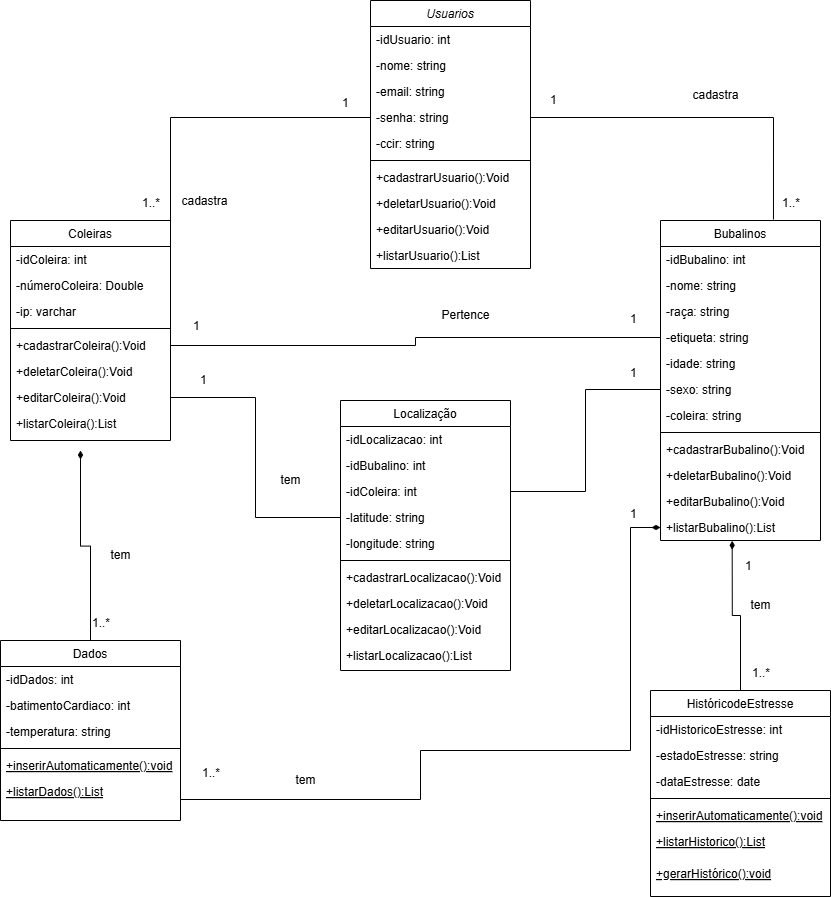
\includegraphics[width=0.95\textwidth]{imgs/bubatag/Diagrama-classe-pi.drawio.png}
   \caption{Diagrama de Classes do Sistema}
   \label{fig:class-diagram}
\end{figure}

\subsection{Diagrama de Objetos}

O diagrama de objetos representa instâncias específicas das classes em determinado momento da execução do sistema. Diferentemente do diagrama de classes, que apresenta uma visão genérica da estrutura do software, o diagrama de objetos demonstra exemplos concretos de objetos e seus relacionamentos.

Esse tipo de diagrama é utilizado para facilitar a visualização do comportamento das entidades e da troca de informações entre os componentes da aplicação.


\begin{figure}[H]
   \centering
   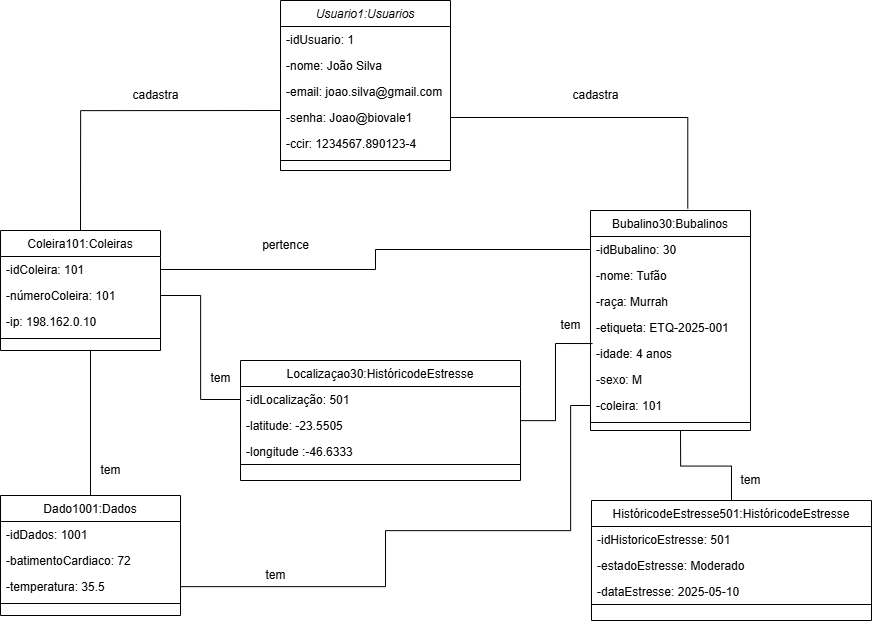
\includegraphics[width=0.95\textwidth]{imgs/bubatag/Diagrama-objeto-pi.drawio.png}
   \caption{Diagrama de Objetos do Sistema}
   \label{fig:object-diagram}
\end{figure}


\subsection{Outros Diagramas UML Importantes}

\begin{itemize}
    \item \textbf{Diagrama de Sequência:} Mostra a interação entre objetos ao longo do tempo
    \item \textbf{Diagrama de Atividades:} Representa o fluxo de trabalho ou processo
    \item \textbf{Diagrama de Componentes:} Mostra a organização física dos componentes
    \item \textbf{Diagrama de Implantação:} Representa a arquitetura física do sistema
    \item \textbf{Diagrama de Estados:} Mostra os estados de um objeto e suas transições
\end{itemize}

% ===== DIAGRAMA DE BANCO DE DADOS =====
\section{Diagrama de Banco de Dados}

O Diagrama de Banco de Dados é uma representação visual da estrutura das informações armazenadas em um sistema \cite{elmasri2019}. Esse tipo de diagrama permite modelar entidades, atributos e relacionamentos existentes no banco de dados, auxiliando no desenvolvimento, manutenção e organização das informações.

Além disso, os diagramas de banco de dados facilitam a compreensão da arquitetura de dados, contribuindo para garantir integridade, consistência e eficiência no armazenamento das informações. Esses diagramas podem ser apresentados utilizando modelos Entidade-Relacionamento (ER) ou modelos relacionais, conforme descrito nas subseções abaixo.

% ===== DIAGRAMA CONCEITUAL =====
\subsection{Diagrama Conceitual}

O diagrama conceitual representa uma visão de alto nível da estrutura do banco de dados \cite{heuser2009}. Nesse modelo são identificadas as entidades principais do sistema, seus atributos e os relacionamentos existentes entre elas, sem considerar detalhes específicos de implementação.

O principal objetivo do modelo conceitual é facilitar a compreensão das regras de negócio e da organização das informações, servindo como base para as etapas posteriores de modelagem do banco de dados.

\begin{figure}[H]
   \centering
   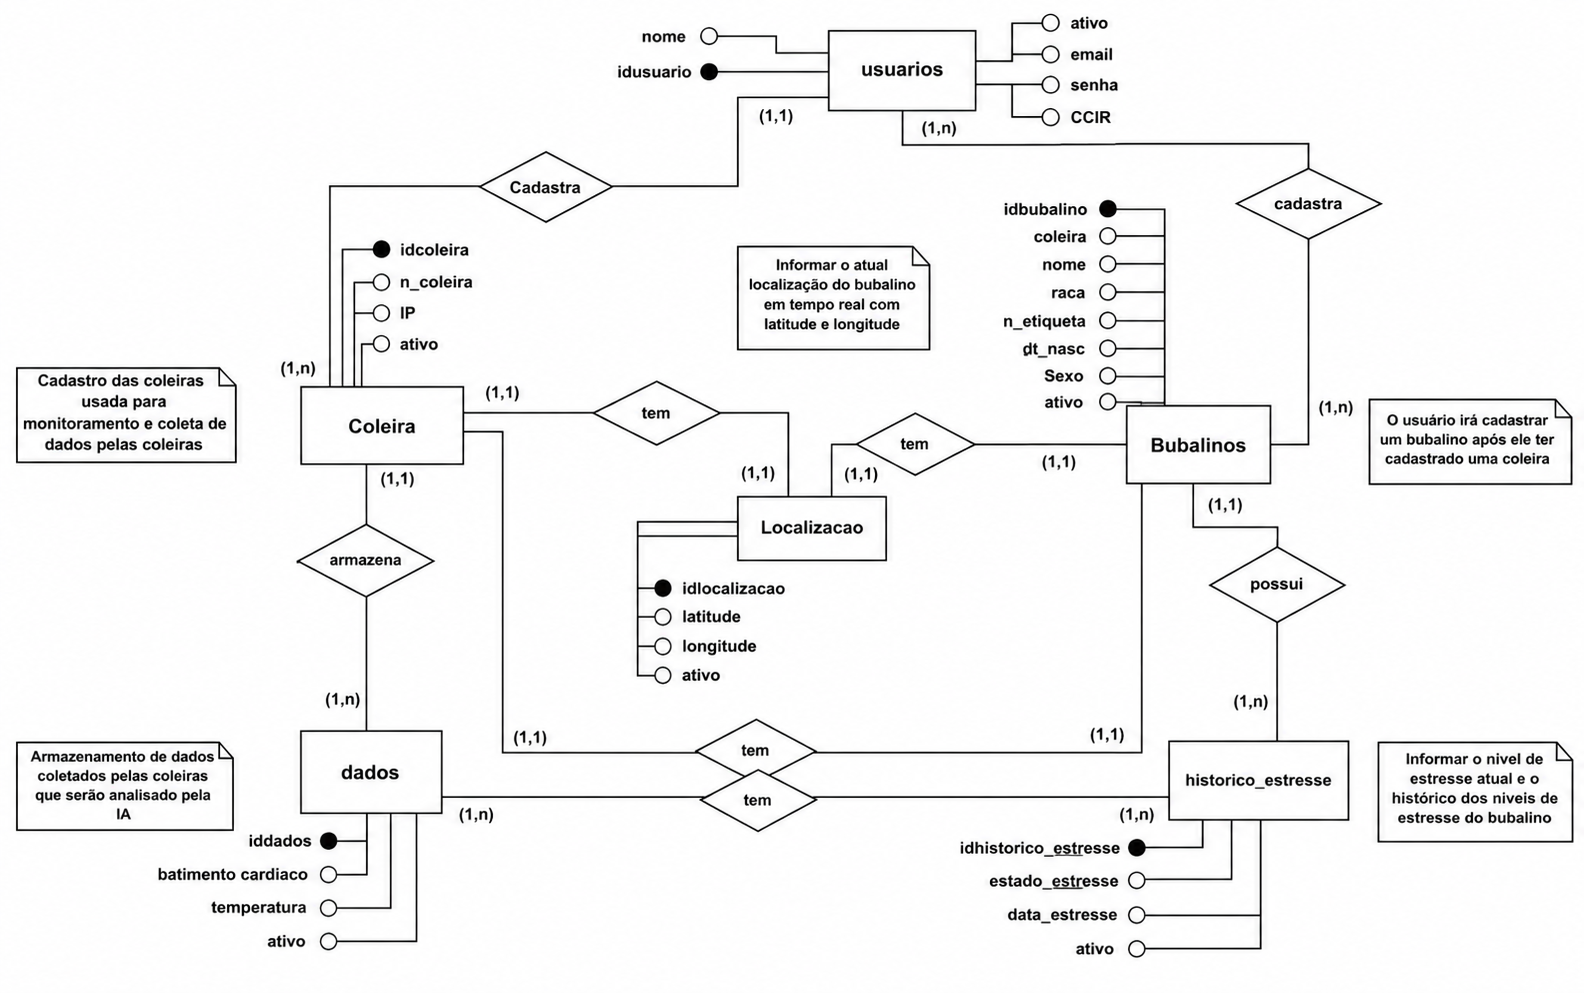
\includegraphics[width=0.9\textwidth]{imgs/bubatag/conceitual.png}
   \caption{Diagrama Conceitual}
   \label{fig:conceitual}
\end{figure}

% ===== DIAGRAMA LÓGICO =====
\subsection{Diagrama Lógico}

O diagrama lógico detalha a estrutura do banco de dados considerando tabelas, atributos, chaves primárias, chaves estrangeiras e relacionamentos entre as entidades \cite{date2020}. Diferentemente do modelo conceitual, o modelo lógico apresenta maior proximidade com a implementação do banco de dados.

Esse modelo é utilizado para organizar os dados de maneira estruturada, garantindo consistência e integridade das informações armazenadas.


\begin{figure}[H]
   \centering
   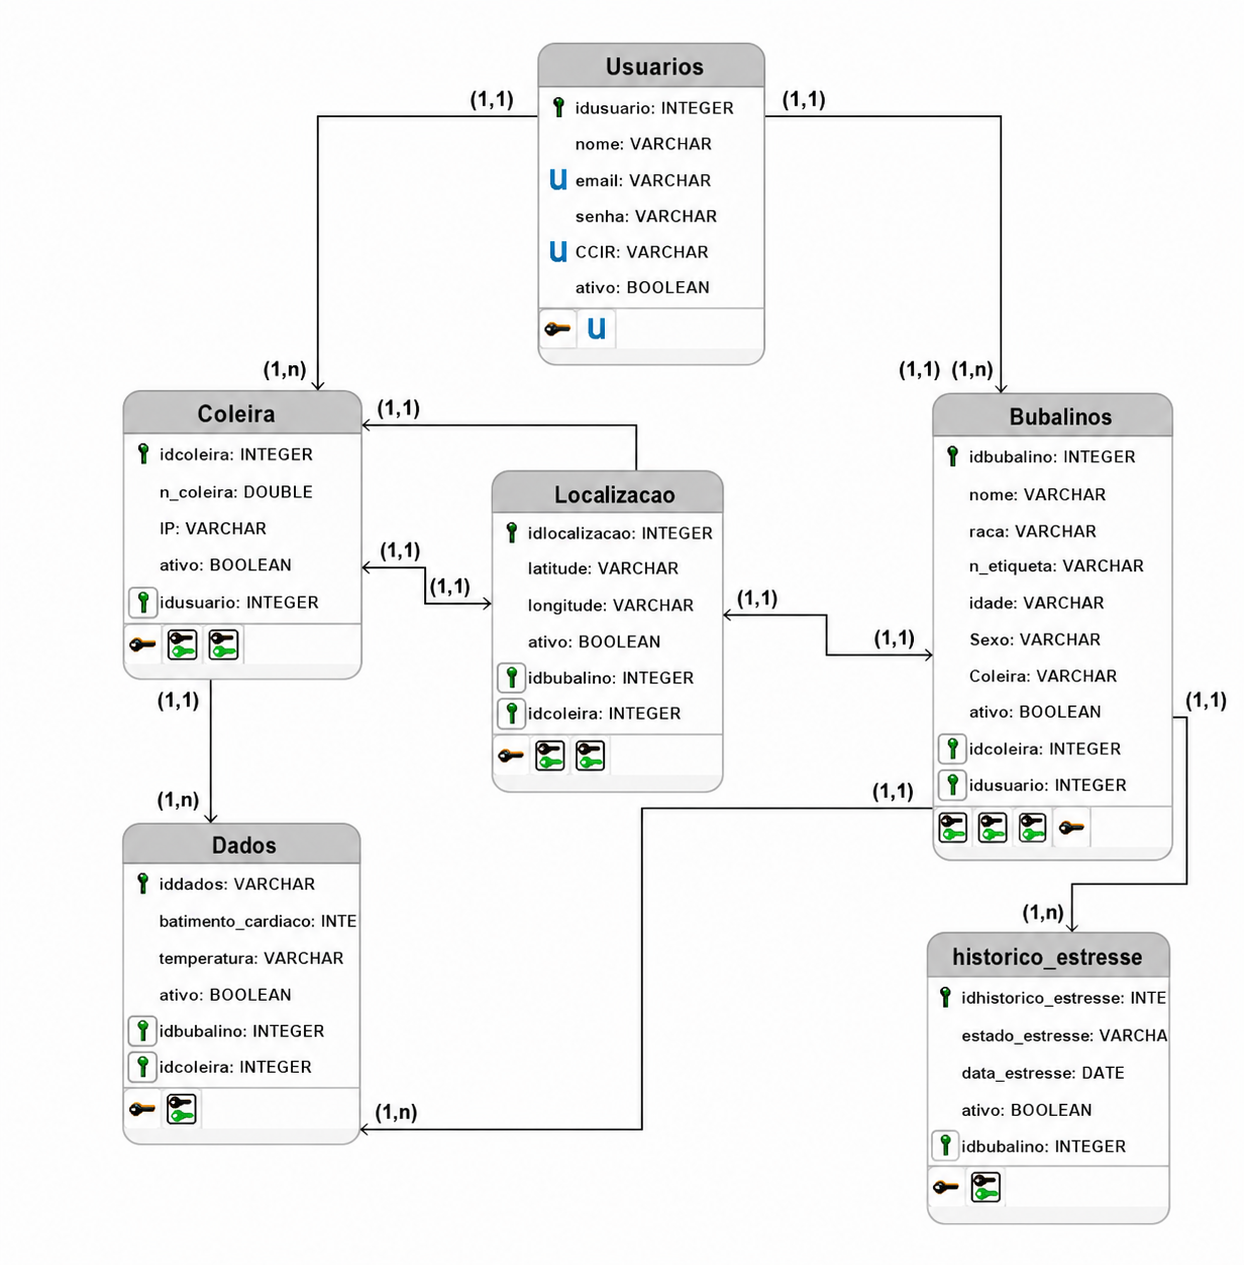
\includegraphics[width=0.9\textwidth]{imgs/bubatag/logico.png}
   \caption{Diagrama Lógico}
   \label{fig:logico}
\end{figure}

% ===== DEVOPS =====
\section{DevOps: Infraestrutura, Automação e Entrega Contínua}

DevOps \cite{wang2023} é uma cultura e conjunto de práticas que integra desenvolvimento de software (Dev) e operações de TI (Ops), focando em automação, colaboração e entrega contínua.

\subsection{Pipeline CI/CD}

O pipeline de integração e entrega contínua é fundamental para automatizar os processos de validação e construção das aplicações:

\begin{figure}[H]
\centering
\begin{tikzpicture}[
    node distance=0.8cm and 0.7cm,
    bloco/.style={
        rectangle,
        draw,
        rounded corners,
        fill=secondarycolor!20,
        text width=2.2cm,
        align=center,
        font=\small,
        minimum height=1cm
    },
    seta/.style={->, thick}
]

\node[bloco] (code) {Push ou Pull Request\\na branch main};
\node[bloco, right=of code] (checkout) {Checkout\\do código};

\draw[seta] (code) -- (checkout);

\node[bloco, above right=0.8cm and 0.7cm of checkout] (api) {Workflow\\API};
\node[bloco, below right=0.8cm and 0.7cm of checkout] (frontend) {Workflow\\Frontend};

\draw[seta] (checkout) -- (api);
\draw[seta] (checkout) -- (frontend);

\node[bloco, right=of api] (syntax) {Verificação sintática\\com Node.js 22};
\node[bloco, right=of syntax] (buildapi) {Construção da\\imagem Docker};
\node[bloco, right=of buildapi] (ghcr) {Publicação da imagem\\no GHCR};

\draw[seta] (api) -- (syntax);
\draw[seta] (syntax) -- (buildapi);
\draw[seta] (buildapi) -- (ghcr);

\node[bloco, right=of frontend] (compose) {Validação do\\Docker Compose};
\node[bloco, right=of compose] (buildfront) {Construção da\\imagem Docker};

\draw[seta] (frontend) -- (compose);
\draw[seta] (compose) -- (buildfront);

\end{tikzpicture}
\caption{Fluxos de CI/CD dos repositórios do Bubatag}
\label{fig:cicd}
\end{figure}

\subsection{Exemplo de Configuração CI/CD}

Os processos de integração contínua do Bubatag são automatizados por meio do GitHub Actions, utilizando arquivos YAML armazenados no diretório \texttt{.github/workflows} de cada repositório.

No frontend, o workflow é acionado por eventos de \textit{push} e \textit{pull request} direcionados à branch \texttt{main}. Suas etapas incluem a obtenção do código-fonte, a configuração do Docker Buildx, a validação do arquivo Docker Compose e a construção da imagem Docker da aplicação.

A seguir, apresenta-se a configuração utilizada no repositório do frontend:

\begin{verbatim}
name: CI/CD - Bubatag Frontend

on:
  push:
    branches:
      - main
  pull_request:
    branches:
      - main

jobs:
  build:
    runs-on: ubuntu-latest

    steps:
      - name: Baixar código
        uses: actions/checkout@v4

      - name: Configurar Docker Buildx
        uses: docker/setup-buildx-action@v3

      - name: Validar Docker Compose
        run: docker compose -f ./sistema-front/docker-compose.yml config

      - name: Construir imagem do frontend
        run: docker compose -f ./sistema-front/docker-compose.yml build
\end{verbatim}

Na API, o workflow também é acionado por eventos de \textit{push} e \textit{pull request} direcionados à branch \texttt{main}. O processo realiza a configuração do ambiente Node.js 22, a instalação das dependências, a verificação sintática do código, a construção da imagem Docker e sua publicação no GitHub Container Registry (GHCR).

A configuração utilizada no repositório da API é apresentada a seguir:

\begin{verbatim}
name: CI/CD - Bubatag API

on:
  push:
    branches:
      - main
  pull_request:
    branches:
      - main

permissions:
  contents: read
  packages: write

jobs:
  build:
    runs-on: ubuntu-latest

    steps:
      - name: Baixar código
        uses: actions/checkout@v4

      - name: Configurar Node.js
        uses: actions/setup-node@v4
        with:
          node-version: 22
          cache: npm

      - name: Instalar dependências
        run: npm ci

      - name: Validar sintaxe
        run: node --check src/server.js

      - name: Construir imagem Docker
        run: docker build -t bubatag-api .

      - name: Login no GitHub Container Registry
        uses: docker/login-action@v3
        with:
          registry: ghcr.io
          username: \${{ github.actor }}
          password: \${{ secrets.GITHUB_TOKEN }}

      - name: Publicar imagem Docker
        run: |
          docker tag bubatag-api ghcr.io/\${{ github.repository_owner }}/bubatag-api:latest
          docker push ghcr.io/\${{ github.repository_owner }}/bubatag-api:latest
\end{verbatim}

Dessa forma, os dois repositórios possuem processos automatizados de integração contínua. Enquanto o frontend realiza a validação da configuração do Docker Compose e a construção de sua imagem, a API também automatiza a instalação de dependências, a verificação sintática e a publicação da imagem Docker no GHCR.

\subsection{Infraestrutura como Código}

A infraestrutura do projeto Bubatag utiliza ferramentas de controle de versão, automação de processos e containerização, que auxiliam no gerenciamento e na construção das aplicações. A Tabela \ref{tab:devops-tools} apresenta as principais ferramentas utilizadas.

\begin{table}[H]
\centering
\caption{Ferramentas DevOps Utilizadas}
\label{tab:devops-tools}
\begin{tabular}{|l|l|p{6cm}|}
\hline
\textbf{Categoria} & \textbf{Ferramenta} & \textbf{Finalidade} \\
\hline
Controle de Versão & Git + GitHub & Versionamento e gerenciamento do código-fonte \\
CI/CD & GitHub Actions & Automação das etapas de validação e construção das aplicações \\
Containerização & Docker & Construção e empacotamento das aplicações em containers \\
Orquestração & Docker Compose & Configuração e execução de serviços containerizados \\
Registro de Imagens & GitHub Container Registry (GHCR) & Armazenamento e publicação da imagem Docker da API \\
\hline
\end{tabular}
\end{table}

\subsection{Infraestrutura do Sistema}

Esta seção apresenta a infraestrutura do sistema Bubatag, considerando os componentes de hardware, comunicação, armazenamento e aplicações utilizados no desenvolvimento do protótipo. A arquitetura permite a coleta de dados fisiológicos dos animais, seu envio para uma API e a disponibilização das informações nas interfaces web e mobile.

\subsection{Arquitetura de Rede}

A infraestrutura do Bubatag é organizada em componentes responsáveis pela coleta, transmissão, processamento e visualização dos dados. A Tabela \ref{tab:infrastructure} apresenta os principais componentes da arquitetura.

\begin{table}[H]
\centering
\caption{Componentes de Infraestrutura do Bubatag}
\label{tab:infrastructure}
\begin{tabular}{|l|p{10cm}|}
\hline
\textbf{Componente} & \textbf{Descrição} \\
\hline

\textbf{Dispositivos e Rede Local} &
\begin{itemize}[leftmargin=*, nosep]
    \item Microcontrolador ESP32 responsável pela coleta e transmissão dos dados
    \item Sensor DS18B20 para medição da temperatura
    \item Sensor MAX30102 para leitura da frequência cardíaca
    \item Comunicação Wi-Fi para envio das informações à API
    \item Utilização de conexão sem fio para comunicação entre os dispositivos
\end{itemize} \\
\hline

\textbf{Infraestrutura em Nuvem} &
\begin{itemize}[leftmargin=*, nosep]
    \item API REST hospedada na plataforma Render
    \item Banco de dados não relacional MongoDB para armazenamento das informações
    \item Recebimento e processamento das leituras de telemetria
    \item Serviço experimental de Inteligência Artificial para classificação dos dados fisiológicos e geração de relatórios
    \item Comunicação entre os dispositivos e as aplicações por meio de requisições HTTP
\end{itemize} \\
\hline

\textbf{Aplicações Web e Mobile} &
\begin{itemize}[leftmargin=*, nosep]
    \item Interface web desenvolvida com React para visualização e gerenciamento das informações
    \item Aplicação mobile destinada ao acompanhamento dos animais
    \item Visualização de dados de temperatura, frequência cardíaca e localização
    \item Integração das aplicações com a API REST
    \item Utilização de mapas para apresentação dos registros de localização dos animais
\end{itemize} \\
\hline

\textbf{Automação e Segurança} &
\begin{itemize}[leftmargin=*, nosep]
    \item Controle de versão dos repositórios utilizando Git e GitHub
    \item Automação de processos de integração contínua com GitHub Actions
    \item Construção e execução de aplicações em containers utilizando Docker
    \item Publicação da imagem Docker da API no GitHub Container Registry (GHCR)
    \item Comunicação entre os componentes por meio de endpoints da API
\end{itemize} \\
\hline

\end{tabular}
\end{table}

\subsection{Diagrama de Infraestrutura}

Para ilustrar a organização dos componentes e o fluxo de comunicação entre os dispositivos, a API, o banco de dados e as aplicações, apresenta-se o diagrama de infraestrutura do sistema Bubatag.

\begin{figure}[H]
\centering
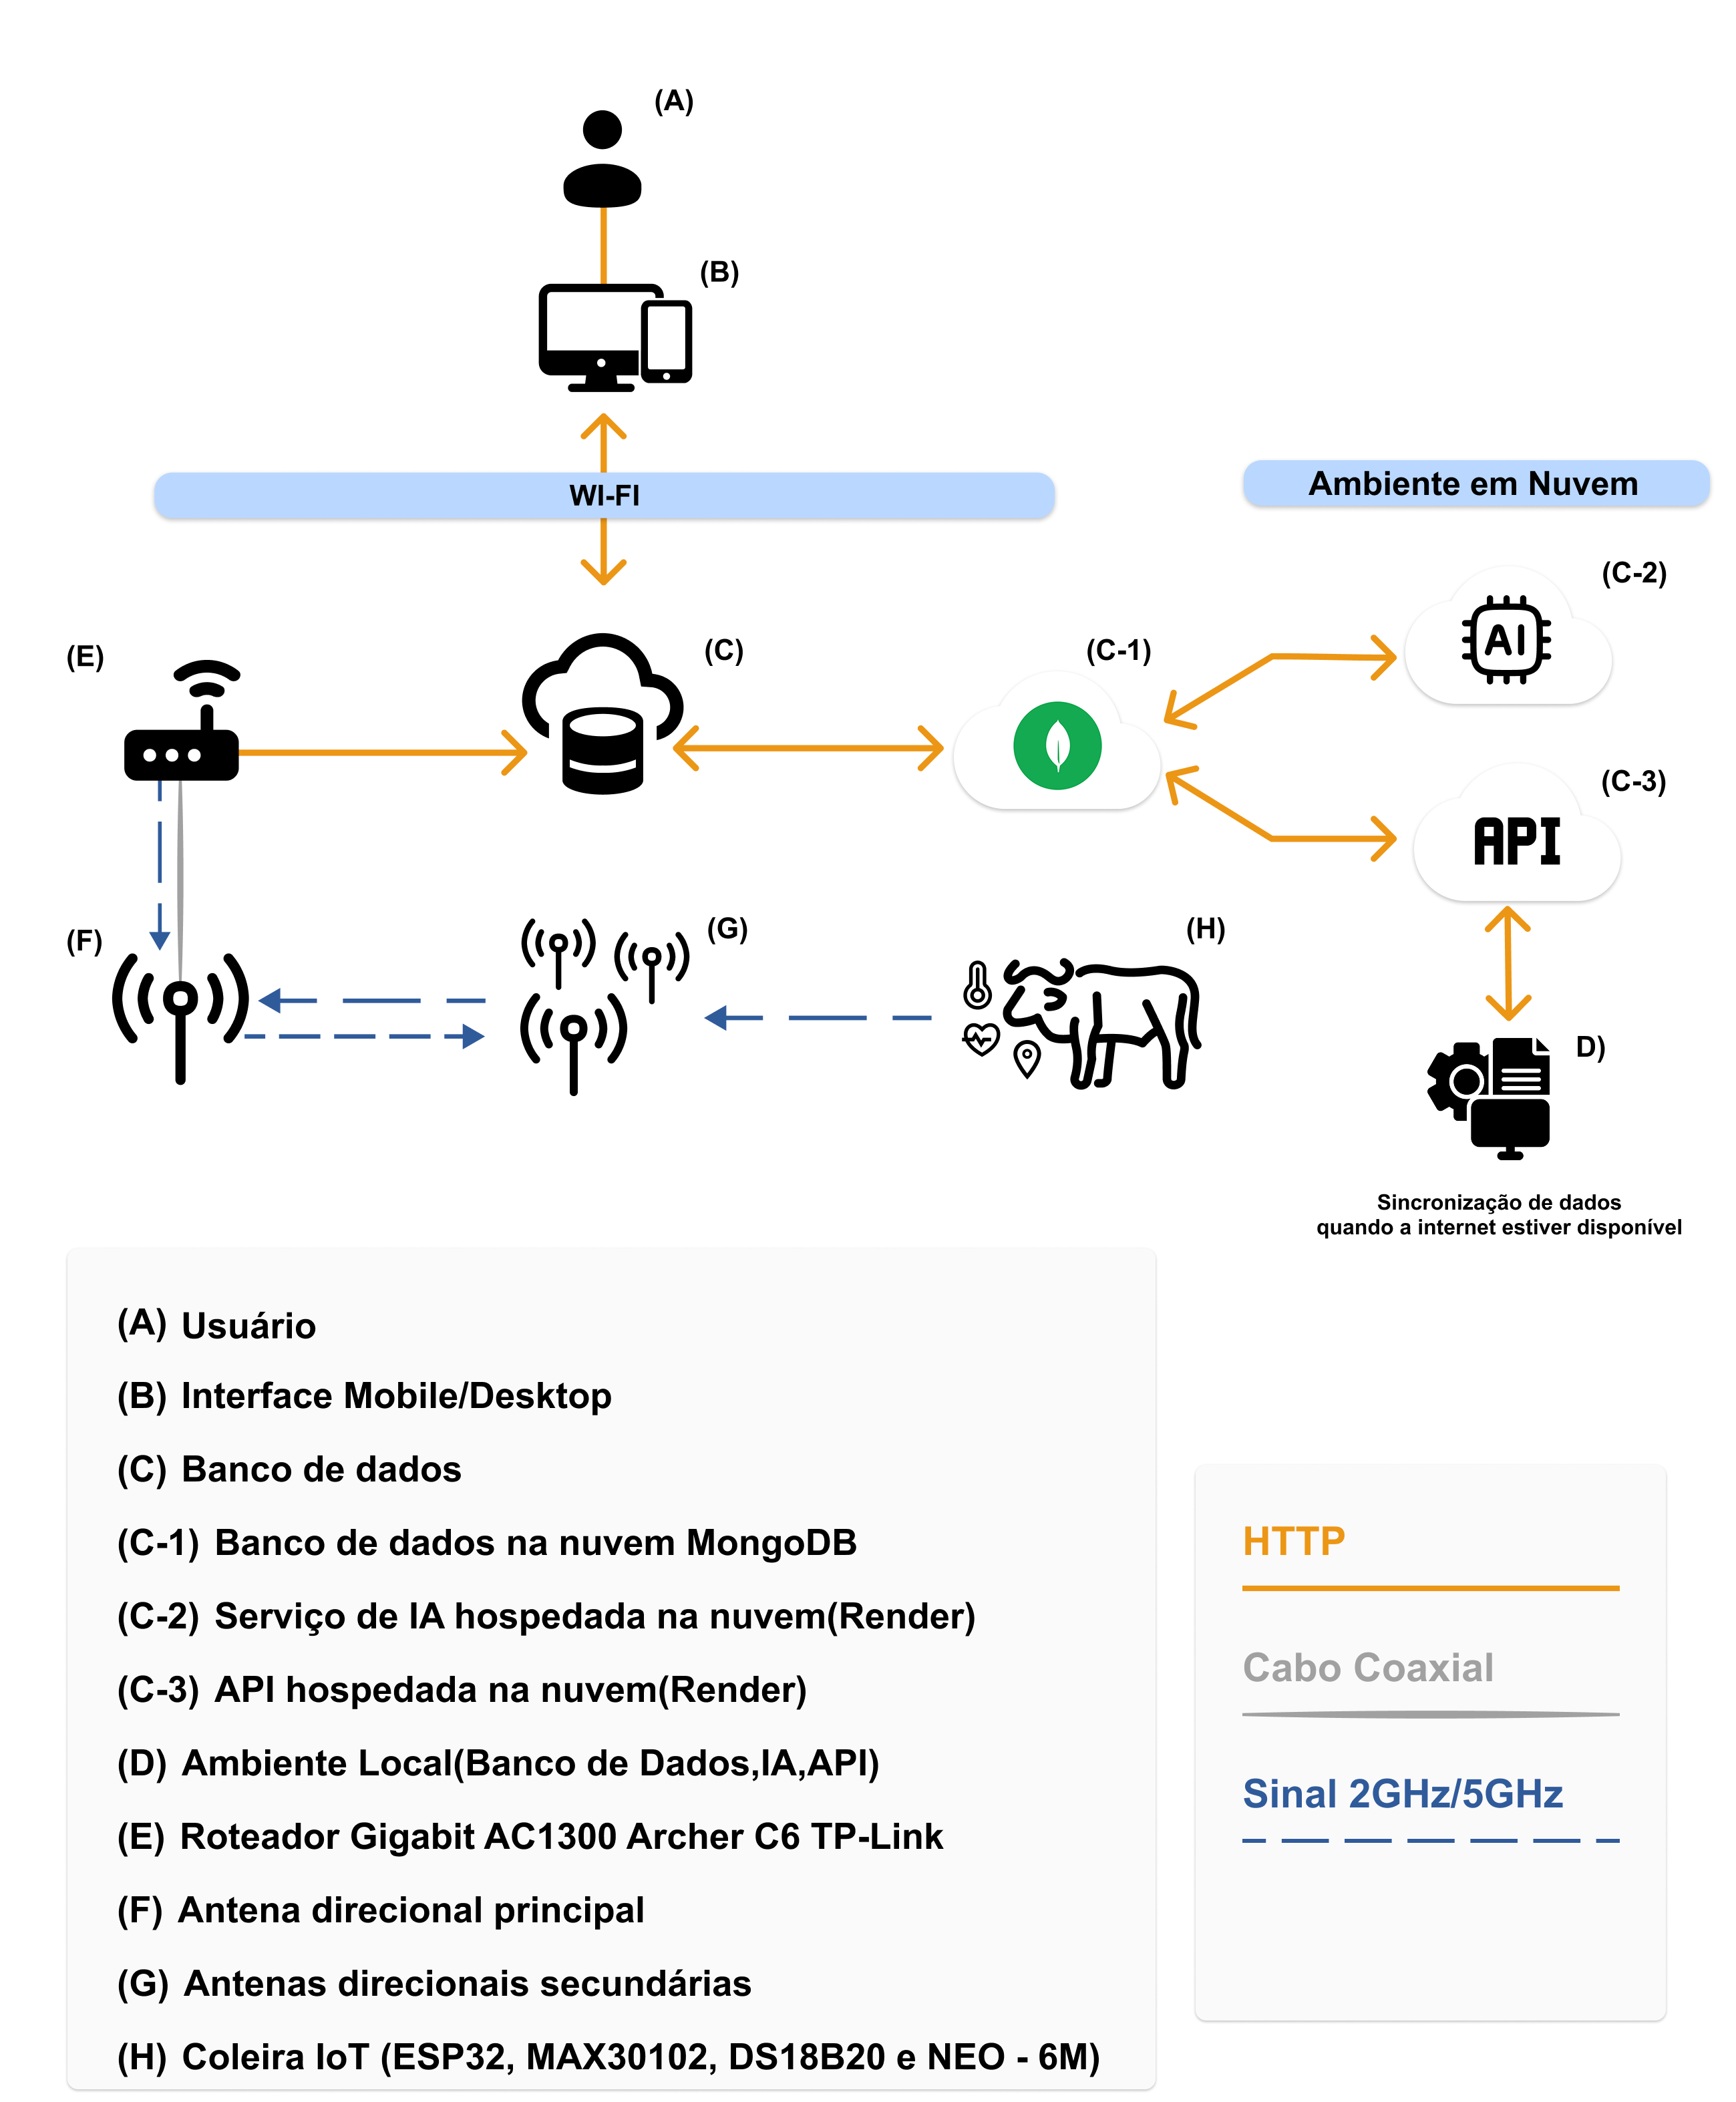
\includegraphics[width=\textwidth]{imgs/bubatag/DIAGRAMA DE REDE - ARTIGO.png}
\caption{Diagrama de Infraestrutura do Sistema Bubatag}
\label{fig:infrastructure-diagram}
\end{figure}

A arquitetura apresentada é composta pelos seguintes elementos:

\begin{itemize}
    \item \textbf{Coleiras Inteligentes:} Dispositivos responsáveis pela coleta de dados fisiológicos dos animais, utilizando o microcontrolador ESP32 conectado aos sensores DS18B20, para medição da temperatura, e MAX30102, para leitura da frequência cardíaca.

    \item \textbf{Comunicação Wi-Fi:} Utilizada para estabelecer a comunicação entre o ESP32 e a API, permitindo o envio das informações coletadas pelos sensores.

    \item \textbf{API REST:} Responsável por receber as informações de telemetria, processar as requisições e intermediar a comunicação entre os dispositivos, o banco de dados e as aplicações.

    \item \textbf{Banco de Dados MongoDB:} Banco de dados não relacional utilizado para armazenar as informações dos usuários, animais, coleiras, leituras fisiológicas, registros de localização e histórico de estresse.

    \item \textbf{Servidor em Nuvem:} Ambiente responsável por disponibilizar a API e permitir o acesso remoto aos serviços do sistema. Atualmente, a API está hospedada na plataforma Render.

    \item \textbf{Inteligência Artificial (IA):} Serviço experimental responsável pela classificação dos dados fisiológicos dos animais em categorias de estresse e pelo apoio à geração de relatórios. O modelo encontra-se em desenvolvimento e utiliza dados simulados em sua etapa experimental.

    \item \textbf{Aplicação Web:} Interface desenvolvida para permitir o gerenciamento do rebanho, a consulta das informações dos animais e a visualização dos dados fisiológicos e registros de localização em mapas.

    \item \textbf{Aplicação Mobile:} Interface destinada ao acompanhamento dos animais por dispositivos móveis. Sua integração com a API e o banco de dados encontra-se em desenvolvimento.
\end{itemize}

\subsection{Arquitetura de Deploy}

A arquitetura de deploy do Bubatag utiliza o GitHub Actions para automatizar etapas de validação, construção e publicação das aplicações. Os processos são definidos separadamente para os repositórios do frontend e da API, conforme apresentado na Figura \ref{fig:deployment}.

\begin{figure}[H]
\centering
\begin{tikzpicture}[
    node distance=0.8cm and 0.7cm,
    component/.style={
        rectangle,
        draw,
        rounded corners,
        fill=secondarycolor!20,
        text width=3.2cm,
        align=center,
        font=\small,
        minimum height=1cm
    },
    seta/.style={->, thick}
]

% Repositórios
\node[component] (github) {GitHub\\Repositórios do Bubatag};

% Separação dos workflows
\node[component, below left=1cm and 0.5cm of github] (front) {Workflow Frontend\\GitHub Actions};
\node[component, below right=1cm and 0.5cm of github] (api) {Workflow API\\GitHub Actions};

\draw[seta] (github) -- (front);
\draw[seta] (github) -- (api);

% Fluxo do Frontend
\node[component, below=of front] (compose) {Validação do\\Docker Compose};
\node[component, below=of compose] (buildfront) {Construção da\\Imagem Docker};

\draw[seta] (front) -- (compose);
\draw[seta] (compose) -- (buildfront);

% Fluxo da API
\node[component, below=of api] (node) {Node.js 22\\Instalação e validação};
\node[component, below=of node] (buildapi) {Construção da\\Imagem Docker};
\node[component, below=of buildapi] (ghcr) {GitHub Container Registry\\(GHCR)};

\draw[seta] (api) -- (node);
\draw[seta] (node) -- (buildapi);
\draw[seta] (buildapi) -- node[right, font=\scriptsize]{Publicação} (ghcr);

% Hospedagem da API
\node[component, below=of ghcr] (render) {Render\\Hospedagem da API};

\draw[seta, dashed] (ghcr) -- node[right, font=\scriptsize]{Hospedagem atual} (render);

\end{tikzpicture}
\caption{Arquitetura de Deploy do Sistema Bubatag}
\label{fig:deployment}
\end{figure}

A arquitetura é composta pelos seguintes elementos:

\begin{itemize}
    \item \textbf{GitHub:} Hospeda os repositórios do projeto, contendo o código-fonte do frontend e da API.

    \item \textbf{GitHub Actions:} Executa os workflows de CI/CD acionados por eventos de \textit{push} e \textit{pull request} na branch principal.

    \item \textbf{Docker:} Responsável pela construção das imagens das aplicações, permitindo seu empacotamento em containers.

    \item \textbf{GitHub Container Registry (GHCR):} Serviço utilizado para armazenar e publicar a imagem Docker da API.

    \item \textbf{Render:} Plataforma de nuvem utilizada para hospedar e executar a API Bubatag.
\end{itemize}

No frontend, o processo automatizado contempla a validação da configuração do Docker Compose e a construção da imagem Docker. Na API, além da configuração do ambiente Node.js e da instalação das dependências, são realizadas a verificação sintática do código, a construção da imagem e sua publicação no GHCR.

Essa estrutura permite organizar os processos de construção e disponibilização das aplicações, facilitando a manutenção e a evolução da infraestrutura do sistema.

\subsection{Métricas e SLA}

O monitoramento de desempenho e disponibilidade é importante para avaliar a confiabilidade e a eficiência da infraestrutura do sistema Bubatag. Para isso, são definidos indicadores que poderão ser utilizados em etapas futuras de testes e validação. Como o projeto ainda se encontra em fase de prototipação, não existem medições sistemáticas suficientes para estabelecer níveis de serviço (SLA) ou metas de desempenho comprovadas.

Entre os principais indicadores propostos, destacam-se:

\begin{itemize}
    \item \textbf{Disponibilidade (Uptime):} Percentual de tempo em que a API e as aplicações permanecem acessíveis.

    \item \textbf{Tempo de Resposta:} Tempo necessário para a API processar uma requisição e retornar uma resposta ao cliente.

    \item \textbf{Taxa de Erro:} Percentual de requisições que resultam em falhas durante a comunicação ou o processamento dos dados.

    \item \textbf{Throughput:} Quantidade de requisições que a API consegue processar por unidade de tempo.

    \item \textbf{Frequência de Deploy:} Quantidade de atualizações disponibilizadas em determinado período, considerando os processos de integração e construção automatizados pelo GitHub Actions.

    \item \textbf{Lead Time:} Tempo decorrido entre a implementação de uma alteração no código e sua disponibilização no ambiente de execução.

    \item \textbf{MTTR (Mean Time to Recovery):} Tempo médio necessário para recuperar o funcionamento do sistema após uma falha.
\end{itemize}

A avaliação desses indicadores permitirá identificar limitações da infraestrutura, acompanhar a evolução do sistema e estabelecer metas de desempenho e disponibilidade compatíveis com as necessidades da bubalinocultura.

\newpage
\section{Conclusão}

Este documento reúne os principais artefatos utilizados na documentação e organização do projeto Bubatag, contemplando aspectos estratégicos, visuais, técnicos e operacionais do desenvolvimento de software.

Os artefatos documentados incluem:

\begin{itemize}
    \item \textbf{CANVAS:} Representação do modelo de negócio e da proposta de valor do Bubatag.

    \item \textbf{SWOT:} Análise estratégica das forças, fraquezas, oportunidades e ameaças relacionadas ao projeto.

    \item \textbf{UX/UI:} Documentação das interfaces e da experiência de uso das aplicações web e mobile.

    \item \textbf{Website:} Estrutura, tecnologias e especificações técnicas da plataforma web.

    \item \textbf{Aplicação:} Descrição das funcionalidades, arquitetura e tecnologias utilizadas no sistema.

    \item \textbf{Diagramas UML:} Representação visual da estrutura, dos componentes e das interações do sistema.

    \item \textbf{Diagramas de Banco de Dados:} Representação da organização e dos relacionamentos entre os dados armazenados no MongoDB.

    \item \textbf{DevOps:} Documentação da infraestrutura, containerização, automação de processos e workflows de integração contínua (CI/CD).
\end{itemize}

A organização desses artefatos proporciona uma visão estruturada do projeto, facilitando a compreensão de sua arquitetura, o acompanhamento do desenvolvimento e a manutenção das aplicações. Além disso, a documentação contribui para a padronização das informações e para a evolução contínua do Bubatag.

\vspace{1cm}
\noindent\rule{\textwidth}{0.5pt}
\vspace{0.3cm}

\newpage
\addcontentsline{toc}{section}{Referências}
\bibliographystyle{abntex2-alf}
\bibliography{referencias}

\end{document}
